\documentclass{article}

\usepackage[final]{neurips_2024}

\usepackage[utf8]{inputenc}
\usepackage[T1]{fontenc}
\usepackage{hyperref}
\usepackage{url}
\usepackage{booktabs}
\usepackage{amsfonts}
\usepackage{nicefrac}
\usepackage{microtype}
\usepackage{xcolor}
\usepackage{graphicx}
\usepackage{amsmath}
\usepackage{amssymb}
\usepackage{tikz}
\usetikzlibrary{arrows.meta,positioning,decorations.pathreplacing,calc}

\title{Where and When Encoder-Decoder Misalignment Signals Feature Absorption in Sparse Autoencoders}

\author{%
  Anonymous Authors \\
  Anonymous Institution \\
  \texttt{anonymous@institution.edu} \\
}

\begin{document}

\maketitle

\begin{abstract}
Feature-based causal analyses built on Sparse Autoencoders (SAEs) silently produce incorrect conclusions when parent latents are suppressed by child latents---a failure mode called feature absorption. Three gaps block systematic progress: detection requires pre-specified probe directions (foreknowledge), generalizability beyond the first-letter spelling task has never been tested, and no actionable structural taxonomy exists. We introduce Encoder-Decoder Alignment (EDA), a weight-only absorption screening metric computable from SAE weight matrices alone without activation data. A formal lower bound derived from the first-order stationarity conditions at a partial minimum of the biconvex sparse dictionary learning (SDL) loss links EDA monotonically to absorption degree. EDA achieves AUROC = 0.776 on Gemma Scope L12-16k (Gemma 2 2B) and AUROC = 0.629 on GPT-2 Small L6 with exact Chanin et al.\ labels, outperforming the decoder cosine baseline by +0.396 AUROC. Attempts to extend absorption measurement to three RAVEL entity-attribute hierarchies (city-continent, city-country, city-language) were falsified by a shuffled hierarchy control: real absorption rates were statistically indistinguishable from shuffled null rates across all 9 tested domain-SAE config combinations (H3 falsified). A three-subtype taxonomy classifies absorbed latents into early absorption (parent decoder direction absent, $\sim$72--75\%), late absorption (encoder suppressed despite decoder presence, $\sim$13\%), and partial absorption (context-dependent, $\sim$13\%). Early-absorption dominance reframes the problem: the dominant failure mode is a training-time dictionary coverage gap, not an inference-time encoder-decoder misalignment. Inference-Time Absorption Correction (ITAC), a training-free proof-of-concept targeting late-type latents, achieves 3.14\% mean false-negative reduction on L12-65k but is structurally inapplicable to the 72--75\% early-type majority. Code is released as an open SAEBench extension.
\end{abstract}

\section{Introduction}

Feature-based causal analyses built on Sparse Autoencoders silently produce incorrect conclusions when parent latents are suppressed by child latents---a failure mode called \textbf{feature absorption} \cite{chanin2024absorption}. Sparse Autoencoders decompose neural network activations into sparse combinations of learned features, enabling researchers to inspect and steer individual computational units inside language models \cite{bricken2023monosemanticity,cunningham2023sparse}. SAEBench evaluates hundreds of SAEs across models and architectures, confirming that dictionary learning produces interpretable features at scale \cite{karvonen2025saebench}. Yet absorption persistently undermines SAE reliability.

Feature absorption occurs when a parent latent---one encoding a general concept---is suppressed to zero on inputs where a more specific child latent is active, even though the parent concept is present in the input \cite{chanin2024absorption}. Consider a concrete example (Figure~\ref{fig:mechanism}a): a latent trained to detect ``starts-with-A words'' (parent) fails to fire whenever a ``starts-with-A proper nouns'' latent (child) is active. The child's activation absorbs the parent's reconstruction contribution; the parent latent reads as inactive despite the input containing an A-word. This suppression is a systematic consequence of sparsity pressure during training: the biconvex SDL loss rewards solutions where one latent handles a subset of inputs that two latents previously shared \cite{tang2025unified}.

Absorption is not confined to toy models. SAEBench measurements confirm the phenomenon across Gemma Scope SAEs at multiple layers and dictionary widths \cite{karvonen2025saebench}, and it has motivated architectural responses including OrtSAE, Matryoshka SAE, KronSAE, MP-SAE, and masked regularization \cite{narayanaswamy2026masked,costa2025mpsae}. The practical consequence is severe: any feature-based causal analysis or steering experiment that reads parent latent activations will silently produce incorrect conclusions on inputs where a child latent is active.

Despite sustained attention, three gaps remain open. \textbf{Gap 1---Detection requires foreknowledge.} The Chanin et al.\ metric, the only quantitative absorption measure, requires pre-specified probe directions: you must already know which parent-child hierarchy to test before you can measure absorption. \textbf{Gap 2---Generalizability is assumed, not tested.} Every published absorption measurement uses the first-letter spelling task. \textbf{Gap 3---No actionable taxonomy.} All absorbed latents are treated as a single category, yet structurally distinct failure modes require different remediation paths.

This paper addresses all three gaps within a unified, training-free framework. Our contributions are:

\begin{enumerate}
\item \textbf{Encoder-Decoder Alignment (EDA)}, a weight-only absorption screening metric computable from SAE weight matrices alone without activation data (Figure~\ref{fig:mechanism}b). We derive a formal lower bound from the first-order stationarity conditions at a partial minimum of the biconvex SDL loss (Theorem~1) linking EDA monotonically to absorption degree. EDA achieves AUROC = 0.776 on Gemma Scope L12-16k, outperforming the decoder cosine baseline by +0.396 AUROC (DeLong $p \approx 0$).

\item \textbf{Cross-domain generalization: a null result with conditional evidence.} We test whether absorption generalizes beyond the first-letter task to three RAVEL entity-attribute hierarchies. A proper shuffled hierarchy control shows real absorption rates are statistically indistinguishable from shuffled null rates (0/9 domain-SAE config combinations pass; H3 falsified). The null result is attributable to below-quality-gate bridge-model probes (accuracy 37--71\% vs.\ required 85\%); we preserve the finding as a pending contribution requiring same-model probe access.

\item \textbf{Three-subtype absorption taxonomy.} We classify absorbed latents into early absorption (parent decoder direction absent; $\sim$72--75\% of cases), late absorption (parent direction present but encoder suppressed; $\sim$13\%), and partial absorption (context-dependent selective failure; $\sim$13\%). Early-absorption dominance reveals that the dominant failure mode is a training-time dictionary coverage gap, not encoder suppression.
\end{enumerate}

We additionally introduce Inference-Time Absorption Correction (ITAC), a training-free proof-of-concept for late-type latents achieving 3.14\% mean false-negative reduction on L12-65k. We also report a negative scaling result: wider SAEs absorb more at matched $L_0$, ruling out a simple width-based mitigation.

\section{Background and Related Work}

\subsection{Sparse Autoencoders for Mechanistic Interpretability}

Transformer-based language models encode many more concepts than they have dimensions, representing features as overlapping linear directions in a phenomenon called \textit{superposition} \cite{elhage2022toy}. Sparse Autoencoders decompose these entangled residual stream activations $x \in \mathbb{R}^{d_{\text{model}}}$ into sparse combinations of learned features by optimizing the sparse dictionary learning (SDL) loss:
\begin{equation}
\mathcal{L}(\theta) = \mathbb{E}_x \left[\|x - \hat{x}\|^2 + \lambda \|z\|_1\right], \quad \text{s.t.} \quad \|d_j\| = 1 \; \forall j.
\tag{1}
\end{equation}
The biconvex SDL loss is convex separately in the encoder parameters $W_e$ and the decoder parameters $W_d$, but not jointly, producing a landscape of partial minima that underlies absorption \cite{tang2025unified}.

Early demonstrations showed SAEs recover interpretable, approximately monosemantic features \cite{bricken2023monosemanticity}. Subsequent scaling to frontier models \cite{templeton2024scaling,gao2024scaling} produced SAEs with millions of latents. Architectural improvements include Gated SAEs \cite{rajamanoharan2024gated}, JumpReLU SAEs \cite{rajamanoharan2024jumprelu}, and TopK SAEs \cite{gao2024scaling}. The Gemma Scope suite provides 400+ pre-trained SAEs \cite{lieberum2024gemma}, and SAEBench standardizes evaluation across eight metrics \cite{karvonen2025saebench}.

Three recent papers challenge SAE reliability: Cui et al.\ \cite{cui2025limits} provide closed-form analysis showing SAEs generally fail to recover ground-truth features unless features are extremely sparse. Korznikov et al.\ \cite{korznikov2026sanity} find trained SAEs recover only 9\% of true features in synthetic settings. Song et al.\ \cite{song2025consistency} show SAE features are inconsistent across training runs (TopK SAEs: PW-MCC = 0.80).

\subsection{Feature Absorption: Definition and Prior Work}

Chanin et al.\ \cite{chanin2024absorption} define feature absorption as the systematic failure of a parent latent to activate when its child latent is active, even though the parent concept is present in the input. Chanin et al.\ validate this mechanism on a toy model and measure absorption rates of 15--35\% across Gemma Scope SAEs at widths 16k and 65k.

Tang et al.\ \cite{tang2025unified} provide theoretical grounding: at partial minima, the encoder direction $w_{e,j}$ for an absorbed parent latent shifts away from its decoder direction $d_j$ by incorporating child decoder components. Several architectural responses aim to reduce absorption: Matryoshka SAEs \cite{bussmann2025matryoshka} train nested dictionaries simultaneously; OrtSAE \cite{korznikov2025ortsae} enforces pairwise decoder orthogonality, reducing absorption by 65\%; masked regularization \cite{narayanaswamy2026masked} disrupts co-occurrence patterns; MP-SAE \cite{costa2025mpsae} uses iterative encoding. All of these require retraining the SAE.

\subsection{RAVEL and Entity-Attribute Hierarchies}

The RAVEL dataset \cite{huang2024ravel} provides structured entity-attribute pairs for probing factual representations. City-continent, city-country, and city-language hierarchies define natural parent-child feature structures analogous to the first-letter task. RAVEL has been adopted in SAEBench as a separate evaluation metric, but no prior work has used it to measure feature absorption.

\section{Encoder-Decoder Alignment (EDA) as an Absorption Indicator}

The Chanin et al.\ metric requires pre-specified probe directions and activation data. We seek a complementary screening signal computable from SAE weights alone.

\subsection{Derivation}

When no absorption is present and the SAE is at a partial minimum, latent $j$'s encoder direction $w_{e,j}$ (row $j$ of $W_e$) aligns with its decoder direction $d_j$. Absorption disrupts this alignment. When a child latent $c$ absorbs the parent latent $j$, the encoder direction $w_{e,j}$ rotates away from $d_j$ because the sparsity penalty drives $z_j$ toward zero on inputs where $z_c > 0$.

This geometric observation motivates a scalar metric:
\begin{equation}
\text{EDA}(j) = 1 - \cos(w_{e,j}, d_j) = 1 - \frac{w_{e,j} \cdot d_j}{\|w_{e,j}\| \cdot \|d_j\|}.
\tag{2}
\end{equation}
EDA ranges from 0 (perfect alignment) to 2 (perfect anti-alignment). It requires only the SAE weight matrices $W_e$ and $W_d$---no activation data, no probe directions, no model forward passes.

\subsection{Formal Lower Bound (Theorem 1)}

\textbf{Theorem 1 (EDA Lower Bound).} \textit{For a Sparse Autoencoder at a partial minimum of the biconvex SDL loss (Equation~1), if latent $j$ exhibits $\delta$-absorption of child $c$ (where $\delta \geq 0$ is the magnitude of encoder suppression due to child $c$), then:}
\begin{equation}
\text{EDA}(j) \geq \frac{\delta^2 \sin^2(\theta_{jc})}{2 + \delta^2},
\tag{3}
\end{equation}
\textit{where $\theta_{jc}$ is the angle between decoder directions $d_j$ and $d_c$.}

The bound is monotonically increasing in $\delta$: stronger absorption produces larger EDA. The $\sin^2(\theta_{jc})$ factor means the bound is tightest when the parent and child decoder directions are orthogonal.

\textit{Proof sketch.} At a partial minimum, absorption introduces a perturbation: the gradient contribution from child-active inputs pushes $w_{e,j}$ away from $d_j$ by an amount proportional to $\delta \cdot \|d_c\| \sin(\theta_{jc})$ when projected perpendicular to $d_j$, yielding a residual with magnitude $\geq \delta \sin(\theta_{jc})$. Converting to cosine distance gives the quadratic form in Equation~(3).

\subsection{D-EDA: Directional Decomposition}

Scalar EDA measures the magnitude of encoder-decoder misalignment but does not reveal its cause. Directional EDA (D-EDA) decomposes the misalignment residual to distinguish absorption from polysemanticity.

\textbf{Step 1:} Compute the residual $r_j = w_{e,j} - \frac{w_{e,j} \cdot d_j}{\|d_j\|^2} d_j$.

\textbf{Step 2:} Decompose $r_j$ in the decoder dictionary via sparse regression: $r_j \approx \sum_k \beta_k d_k$, minimizing $\|r_j - W_d \beta\|^2 + \mu \|\beta\|_1$ with $\mu = 0.01$.

\textbf{Step 3:} The absorption signature is sparse $\beta$ with the active components $k$ satisfying $\cos(d_k, d_j) > 0.1$.

D-EDA does not outperform scalar EDA on Gemma Scope SAEs (Section~4) due to ill-conditioning when $d_{\text{SAE}} \gg d_{\text{model}}$ (see Appendix~\ref{sec:deda_ill} for details). One exception: GPT2-L10, where D-EDA achieves AUROC = 0.762 [0.686, 0.830] where scalar EDA achieves only 0.336.

\subsection{Synthetic Validation (SynthSAEBench)}

We validate EDA under controlled conditions using SynthSAEBench (construction details in Appendix~\ref{sec:synthasb}): five synthetic SAEs with $d_{\text{model}} = 64$, $d_{\text{SAE}} = 500$, and 100 designated absorbed features.

As shown in Figure~\ref{fig:synthsae}, EDA achieves perfect discrimination on synthetic data: AUROC = 1.000 and best-threshold F1 = 0.974. Absorbed latents have median EDA = 0.837 versus non-absorbed median EDA = 0.069---a $12\times$ separation ratio.

\begin{figure}[t]
\centering
\includegraphics[width=0.90\linewidth]{figures/fig2_synthsae.pdf}
\caption{SynthSAEBench validation: (a) ROC curve showing perfect discrimination (AUROC = 1.000); (b) EDA distributions for absorbed (median = 0.84) vs.\ non-absorbed (median = 0.07) synthetic latents. Five trials, 500 features each, 100 absorbed per trial.}
\label{fig:synthsae}
\end{figure}

\section{EDA Validation: Detection Performance}

\subsection{Experimental Setup}

\textbf{Models and SAEs.} We evaluate EDA on two model families. For Gemma 2 2B, we use six Gemma Scope SAEs spanning layers \{5, 12, 19\} and widths \{16k, 65k\} ($d_{\text{SAE}} \in \{16384, 65536\}$). For GPT-2 Small, we use SAELens SAEs at layers 6 and 10 ($d_{\text{SAE}} = 24576$).

\textbf{Ground-truth labels.} For Gemma Scope, labels use Neuronpedia proxy annotations. For GPT-2 Small, we generate exact labels using an adapted \texttt{FeatureAbsorptionCalculator}: logistic regression probes trained on 1,145 words (up to 50 per letter) drawn from a 7,637-word NLTK single-token vocabulary.

\textbf{Metrics.} AUROC is the primary metric, computed with 95\% bootstrap confidence intervals (10,000 resamples, seed = 42). Baseline comparisons use the DeLong test \cite{delong1988}. The pass threshold is AUROC $\geq$ 0.65.

\subsection{Main Results}

Table~\ref{tab:eda_results} reports EDA, D-EDA, decoder cosine baseline, and shuffled EDA null performance across all eight SAE configurations. Figure~\ref{fig:eda_heatmap} visualizes the regime-specific pattern.

\begin{table}[t]
\caption{EDA Detection Performance Across SAE Configurations}
\label{tab:eda_results}
\centering
\small
\begin{tabular}{lcccccccc}
\toprule
Config & Layer & $d_{\text{SAE}}$ & AUROC (EDA) & 95\% CI & AUROC (D-EDA) & AUROC (Dec.\ Cos.) & Cohen's $d$ & Pass \\
\midrule
L5-16k & 5 & 16,384 & \textbf{0.698} & [0.637, 0.779] & 0.602 & 0.302 & 0.764 & PASS \\
L5-65k & 5 & 65,536 & 0.617 & [0.532, 0.725] & 0.534 & 0.383 & 0.385 & FAIL \\
L12-16k & 12 & 16,384 & \textbf{0.776} & [0.700, 0.863] & 0.579 & 0.224 & 1.019 & PASS \\
L12-65k & 12 & 65,536 & 0.468 & [0.315, 0.620] & 0.499 & 0.532 & $-$0.152 & FAIL \\
L19-16k & 19 & 16,384 & 0.458 & [0.317, 0.590] & 0.589 & 0.542 & $-$0.051 & FAIL \\
L19-65k & 19 & 65,536 & 0.562 & [0.438, 0.683] & 0.471 & 0.438 & 0.208 & FAIL \\
GPT2-L6 & 6 & 24,576 & \textbf{0.629} & [0.561, 0.692] & 0.656 & --- & 0.510 & PASS \\
GPT2-L10 & 10 & 24,576 & 0.336 & [0.245, 0.435] & \textbf{0.762} & --- & --- & FAIL \\
\bottomrule
\end{tabular}
\vspace{0.5em}
\par\noindent\footnotesize DeLong test: EDA vs.\ decoder cosine at L5-16k: difference = +0.396, $p \approx 0$; at L12-16k: difference = +0.553, $p \approx 0$.
\end{table}

\begin{figure}[t]
\centering
\includegraphics[width=0.90\linewidth]{figures/fig3_eda_heatmap.pdf}
\caption{EDA AUROC across SAE configurations. Green borders indicate PASS ($\geq$ 0.65). GPT-2 results show EDA and D-EDA side by side.}
\label{fig:eda_heatmap}
\end{figure}

Two of six Gemma Scope configurations pass the AUROC $\geq$ 0.65 threshold: L12-16k (0.776) and L5-16k (0.698). Both are mid-layer, narrow SAEs. EDA cross-validates against SAEBench's precomputed \texttt{encoder\_decoder\_cosine\_sim} with Pearson $r > 0.999$.

\textbf{GPT-2 replication.} GPT2-L6 passes with EDA AUROC = 0.629 (exact labels, $n_{\text{pos}} = 67$). GPT2-L10 reveals a complementary finding: EDA fails (AUROC = 0.336) but D-EDA achieves 0.762 [0.686, 0.830].

\begin{figure}[t]
\centering
\includegraphics[width=0.85\linewidth]{figures/fig4_eda_distributions.pdf}
\caption{EDA distributions for absorbed versus non-absorbed latents at L12-16k and L12-65k. Effect size is large at L12-16k (Cohen's $d$ = 1.019); the group separation inverts at L12-65k due to proxy label noise.}
\label{fig:eda_distributions}
\end{figure}

Figure~\ref{fig:eda_distributions} shows the statistical group separation. At L12-16k, absorbed latents have mean EDA = 0.282 versus 0.214 for non-absorbed (Cohen's $d$ = 1.019, Mann-Whitney $p = 6.4 \times 10^{-5}$).

\subsection{The Pilot-to-Full Discrepancy and Proxy Label Noise}

A pilot run at L12-65k yielded AUROC = 0.853. The full validation collapsed to 0.468---a 0.385 drop. Two factors explain this: the pilot used a capped subset with enriched positive prevalence; the full 65,536-latent evaluation dilutes positives to 0.024\% ($n_{\text{pos}} = 16$). Additionally, Neuronpedia proxy labels introduce systematic noise.

GPT2-L6 with exact Chanin et al.\ labels (AUROC = 0.629, $n_{\text{pos}} = 67$) provides the cleanest validation. EDA is a regime-specific screening tool for mid-layer narrow SAEs, not a universal absorption detector.

\subsection{Polysemanticity Stratification}

At L12-16k, EDA achieves AUROC = 0.922 [0.842, 0.979] on the polysemantic half (above-median feature density, $n_{\text{pos}} = 3$; note: small positive class) versus 0.643 [0.518, 0.763] on the monosemantic half ($n_{\text{pos}} = 13$). The monosemantic AUROC (0.643) better isolates EDA's pure absorption-detection capability.

\section{Cross-Domain Absorption: A Null Result and Conditional Evidence}

\subsection{RAVEL Hierarchy Suite and Probe Limitations}

We tested whether absorption generalizes beyond the first-letter spelling task to three RAVEL entity-attribute hierarchies: city-continent (6 parent classes), city-country ($\sim$100 parent classes), and city-language ($\sim$82 parent classes). \textbf{This hypothesis (H3) was falsified}: a proper shuffled hierarchy control showed real absorption rates are statistically indistinguishable from shuffled null rates.

\textbf{Probe limitations.} We trained logistic regression probes on residual stream activations of Qwen2.5-0.5B ($d_{\text{model}} = 896$) projected to Gemma 2 2B's $d_{\text{model}} = 2304$ via random orthonormal QR decomposition, because Gemma 2 2B remains gated on HuggingFace. Probe accuracy was far below the pre-registered 85\% quality gate: city-continent 71.4\%, city-country 37.8\%, city-language 36.8\%.

\subsection{Shuffled Hierarchy Control: H3 Falsified}

Initial measurements showed all 18 SAE-hierarchy combinations exceeded a 3$\times$ fixed-random-probe baseline. However, this comparison uses fixed random probe directions as denominator---not randomized hierarchy labels---and does not constitute a valid null test for cross-domain absorption.

A proper shuffled hierarchy control randomized parent-child label assignments while holding all other aspects of the pipeline constant. Across all 9 tested domain-SAE config combinations (3 hierarchies $\times$ 3 representative SAE configs), 0 of 9 real-hierarchy absorption rates exceeded the shuffled-label p95 threshold. The pre-registered decision criterion was $\geq$ 1/9 pass; the result is NO\_GO. H3 is recorded as FALSIFIED.

\textbf{Interpretation.} The measured RAVEL signal is a probe-quality artifact. Below-quality-gate probes trained on a different model family and projected via random decomposition do not provide reliable parent-feature directions. Cross-domain generalization of absorption detection remains an open question requiring same-model probe access (Gemma 2 2B or Llama-3.1-8B with gating resolved).

\subsection{Conditional Intra-Domain Coherence (Pending Replication)}

Prior to the shuffled control, we observed high intra-RAVEL coherence across the 6 SAE configurations (city-continent vs.\ city-country: $\rho_s = 0.943$, $p = 0.005$; city-continent vs.\ city-language: $\rho_s = 0.886$, $p = 0.019$; city-country vs.\ city-language: $\rho_s = 0.943$, $p = 0.005$; mean intra-RAVEL $\rho_s = 0.924$). Note that the shuffled control was run on a smaller pilot subset (3 SAE configs) while the coherence analysis used 6 configs; these are separate experiments. The coherence may reflect a genuine SAE-level absorption susceptibility property or a geometric artifact of the bridge-model projection. We retain this as suggestive existence evidence conditional on replication with same-model probes.

\begin{figure}[t]
\centering
\includegraphics[width=0.95\linewidth]{figures/fig5_crossdomain_rates.pdf}
\caption{Absorption rates across 3 RAVEL hierarchies $\times$ 6 SAE configurations (pre-shuffled-control measurements). All 18 measurements exceed the 3$\times$ fixed-random-probe baseline, but a shuffled hierarchy control subsequently falsified this as a probe-quality artifact (0/9 combinations pass the null test; H3 falsified). Rates shown are indicative only.}
\label{fig:crossdomain}
\end{figure}

\begin{figure}[t]
\centering
\includegraphics[width=0.90\linewidth]{figures/fig6_ravel_coherence.pdf}
\caption{Pairwise Spearman $\rho_s$ scatter plots of absorption rates across RAVEL hierarchies (6 SAE configurations per panel). Mean intra-RAVEL $\rho_s = 0.924$. Coherence is suggestive but conditional on replication with same-model probes; the absolute rates are invalidated by the shuffled hierarchy control.}
\label{fig:ravel_coherence}
\end{figure}

The null result and remaining open questions motivate our second contribution: a structural taxonomy of absorbed latents that is independent of probe quality.

\section{Three-Subtype Absorption Taxonomy}

\subsection{Subtype Definitions}

For each absorbed latent $j$ with parent probe direction $v_p$, we apply the decoder coverage criterion with threshold $\tau = 0.3$. Table~\ref{tab:taxonomy} defines the three subtypes.

\begin{table}[t]
\caption{Three-Subtype Taxonomy}
\label{tab:taxonomy}
\centering
\small
\begin{tabular}{lllcc}
\toprule
Subtype & Criterion & EDA Signal & ITAC Remediable & Prevalence (L12-65k) \\
\midrule
\textbf{Early} & $\max_k \cos(d_k, v_p) < \tau$: parent never learned & Low & No & 72.3\% \\
\textbf{Late} & $\max_k \cos(d_k, v_p) \geq \tau$, encoder fails & High & Yes & 13.8\% \\
\textbf{Partial} & $\max_k \cos(d_k, v_p) \geq \tau$, encoder fires sometimes & Intermediate & Partial & 13.8\% \\
\bottomrule
\end{tabular}
\end{table}

\textbf{Early absorption} represents a training-time dictionary coverage failure: the parent feature was never allocated in the SAE dictionary. \textbf{Late absorption} represents an inference-time encoder suppression failure: the parent decoder direction exists but the encoder was trained away from it. \textbf{Partial absorption} is context-dependent.

\subsection{Empirical Distribution}

As shown in Figure~\ref{fig:subtype_eda}, early absorption dominates at both configurations:
\begin{itemize}
\item L12-16k: Early 75.0\%, Late 12.5\%, Partial 12.5\%
\item L12-65k: Early 72.3\%, Late 13.8\%, Partial 13.8\% (Kruskal-Wallis $p = 0.0002$)
\end{itemize}

EDA ordering (late $>$ partial $>$ early) holds at L12-65k (KW $p = 0.0002$). The finding is robust across all 5 tested thresholds (0.20, 0.25, 0.30, 0.35, 0.40).

\begin{figure}[t]
\centering
\includegraphics[width=0.88\linewidth]{figures/fig7_subtype_eda.pdf}
\caption{EDA distributions by absorption subtype at L12-16k and L12-65k. Early-type latents have low EDA (decoder-absent); late-type latents have high EDA (encoder suppressed despite decoder presence). KW $p = 0.0002$ at L12-65k.}
\label{fig:subtype_eda}
\end{figure}

\subsection{The Early-Absorption Dominance Insight}

Early absorption constitutes 72--75\% of all absorbed latents at both tested configurations. This is the paper's central actionable finding: the dominant failure mode is a \textbf{training-time dictionary coverage gap}, not an inference-time encoder-decoder misalignment problem.

This reframing has two direct implications for remediation strategy. First, inference-time corrections such as ITAC are structurally inapplicable to the 75\% early-absorption majority. Second, architectural innovations that directly address dictionary coverage---Matryoshka SAE \cite{bussmann2025matryoshka}, masked regularization \cite{narayanaswamy2026masked}, and MP-SAE \cite{costa2025mpsae}---address the root cause for three-quarters of absorbed latents.

\subsection{ITAC Proof-of-Concept}

Inference-Time Absorption Correction (ITAC) targets the 13\% late-type minority. For a late-type latent $j$ with absorbing child latent $\text{abs}$, ITAC corrects the parent activation as:
\begin{equation}
z_j^{\text{corr}} = \max\!\left(0, \, d_j^\top \!\left(e + z_{\text{abs}} \, d_{\text{abs}}\right)\right),
\tag{6}
\end{equation}
where $e = x - \hat{x}$ is the reconstruction error.

Table~\ref{tab:itac} reports ITAC efficacy. Mean FN reduction at L12-65k: 3.14\% (7.6\% $\to$ 6.2\%), well below the pre-registered 20\% target (H5 falsified). FVU change of $-4.23\%$ confirms no reconstruction quality degradation.

\begin{table}[t]
\caption{ITAC Efficacy by Subtype}
\label{tab:itac}
\centering
\small
\begin{tabular}{llccccc}
\toprule
Config & Subtype & $N$ & FN Before & FN After & FN Reduction & FVU Change \\
\midrule
L12-16k & Late-type & 1 & 0.000 & 0.000 & 0.00\% & +22.11\% \\
L12-65k & Late-type & 10 & 7.6\% & 6.2\% & \textbf{3.14\%} & $-$4.23\% \\
L12-65k & Early/Partial & all & --- & --- & 0.00\% & --- \\
\bottomrule
\end{tabular}
\end{table}

\section{Discussion}

\subsection{EDA as a Regime-Specific Screening Tool}

EDA achieves AUROC = 0.776 at L12-16k and 0.698 at L5-16k on Gemma Scope (Table~\ref{tab:eda_results}), with cross-model confirmation at GPT2-L6 (AUROC = 0.629, exact Chanin et al.\ labels). The operating regime is mid-layer, narrow-dictionary SAEs. At L19-16k (AUROC = 0.458) and L12-65k (AUROC = 0.468), EDA falls to chance-level discrimination.

\textbf{Practical recommendation.} Use EDA to rank latents by absorption risk, then apply the more expensive Chanin et al.\ metric to the top-$k$ high-EDA candidates. At L12-16k, focusing on the top 5\% of latents by EDA contains approximately 56\% of absorbed latents (Prec@50 = 0.0035), reducing the supervised evaluation budget by 20$\times$.

\subsection{Why First-Letter and RAVEL Absorption Do Not Correlate}

The cross-domain analysis reveals striking asymmetry. Within three RAVEL hierarchies, pre-shuffled-control absorption rankings showed high coherence (mean $\rho_s = 0.924$). Between first-letter and RAVEL domains, correlations are negative and non-significant ($\rho_s = -0.20$ to $-0.43$, $p > 0.39$). Three structural differences account for the disconnect: scale incompatibility (SAEBench aggregate fraction vs.\ latent-level rates on different denominators), hierarchy granularity differences (6 vs.\ 100 vs.\ 82 parent classes), and probe-quality degradation from the model proxy. Because the shuffled hierarchy control invalidated the absolute RAVEL rates, both the first-letter vs.\ RAVEL comparison and the intra-RAVEL coherence should be interpreted as suggestive pending same-model probe replication.

\subsection{Negative Results and What They Teach Us}

Four pre-specified hypotheses were falsified, each mechanistically consistent with early-absorption dominance.

\textbf{H3 falsified: RAVEL absorption indistinguishable from shuffled null.} A shuffled hierarchy control (0/9 domain-SAE config combinations pass the null test) invalidated the absolute RAVEL absorption measurements. The signal is attributable to below-quality-gate bridge-model probes (37--71\% accuracy). Cross-domain generalization requires same-model probe access.

\textbf{D-EDA does not outperform scalar EDA on Gemma Scope.} D-EDA achieves AUROC = 0.499--0.602 across all 6 Gemma configurations, consistently below scalar EDA. The exception is GPT2-L10, where D-EDA achieves AUROC = 0.762 versus EDA's 0.336.

\textbf{ITAC achieves 3.14\% mean FN reduction, well below the 20\% target (H5 falsified).} ITAC is geometrically sound but the correction magnitude is insufficient because encoder suppression in late-type latents is more severe than a simple linear projection can recover.

\textbf{H6 falsified: wider SAEs do not show lower absorption at matched $L_0$.} The partial Spearman $\rho(\text{width}, \text{absorption} \mid L_0) = 0.368$ ($p = 0.133$). The log-linear model $\log(\text{absorption}) = -6.45 + 0.59 \cdot \log(\text{width}) - 0.068 \cdot \text{layer}$ achieves $R^2 = 0.167$. The positive width coefficient (0.59) means wider SAEs exhibit weakly higher absorption. Simply scaling SAE width is not a sufficient remedy.

\subsection{Limitations}

\textbf{Proxy labels on Gemma Scope.} All Gemma AUROC values use Neuronpedia-derived proxy labels; definitive validation requires model access. \textbf{RAVEL probe quality below gate.} None of the three RAVEL probes achieve the 85\% accuracy quality gate (city-continent: 71.4\%; city-country: 37.8\%; city-language: 36.8\%). A shuffled hierarchy control confirms the absolute absorption rates are a probe-quality artifact (0/9 domain-SAE config combinations pass). Intra-RAVEL coherence ($\rho_s = 0.924$) remains suggestive but conditional on same-model probe replication. \textbf{ITAC evaluated on synthetic activations only.} Real-activation validation is a necessary next step. \textbf{Limited SAE configurations.} With $n = 6$ Gemma Scope configurations, Spearman correlations have wide confidence intervals.

\section{Conclusion}

This paper addresses three open gaps in feature absorption: detection without foreknowledge, generalizability beyond the first-letter task, and the absence of an actionable taxonomy.

\textbf{EDA as a weight-only screening metric.} $\text{EDA}(j) = 1 - \cos(w_{e,j}, d_j)$ provides a theoretically grounded absorption indicator. Theorem~1 guarantees EDA increases monotonically with absorption degree $\delta$. Empirical validation confirms reliable detection at mid-layer narrow SAEs: AUROC = 0.776 on Gemma Scope L12-16k and AUROC = 0.629 on GPT-2 Small L6 with exact labels.

\textbf{Cross-domain generalization: pending.} An attempt to characterize absorption across three RAVEL entity-attribute hierarchies was invalidated by a shuffled hierarchy control (0/9 domain-SAE combinations pass; H3 falsified). The null result is attributable to below-quality-gate bridge-model probes (37--71\% accuracy vs.\ required 85\%). Intra-RAVEL coherence ($\rho_s = 0.924$) is suggestive but conditional on replication with same-model probes. Cross-domain generalization remains an open question requiring Gemma 2 2B or Llama-3.1-8B probe access.

\textbf{Early-absorption dominance is the central actionable finding.} The three-subtype taxonomy reveals that 72--75\% of absorbed latents are early-type at both L12-16k ($n = 16$) and L12-65k ($n = 65$; KW $p = 0.0002$). The dominant failure mode is a training-time dictionary coverage gap. Targeted architectural solutions such as Matryoshka SAE or masked regularization address the root cause for three-quarters of absorbed latents.

\bibliography{references}
\bibliographystyle{plainnat}

\appendix

\section{SynthSAEBench Construction}
\label{sec:synthasb}

SynthSAEBench is a synthetic benchmark constructed to validate EDA under controlled conditions with known ground-truth absorption labels. Five synthetic SAEs are constructed, each with $d_{\text{model}} = 64$, $d_{\text{SAE}} = 500$ features, and 100 features designated as absorbed.

\textbf{Construction procedure.} Each synthetic SAE is initialized with random unit-normalized decoder columns $d_j$ drawn uniformly from the unit sphere in $\mathbb{R}^{64}$. Encoder directions for non-absorbed latents are set equal to their decoder directions ($w_{e,j} = d_j$, perfect alignment, EDA $= 0$). Absorbed latents are constructed by rotating $w_{e,j}$ away from $d_j$ toward a randomly selected child decoder direction $d_c \neq d_j$:
\begin{equation*}
w_{e,j} = (1-\alpha) d_j + \alpha d_c, \quad \text{normalized to unit length,}
\end{equation*}
where $\alpha \in [0.3, 1.5]$ controls absorption degree $\delta$ (drawn uniformly). This rotation directly implements the geometric mechanism described in Section~3.1.

\textbf{Ground-truth labels.} All 100 rotated latents are labeled absorbed; the remaining 400 are labeled non-absorbed. No label noise is added.

\section{D-EDA Ill-Conditioning Analysis}
\label{sec:deda_ill}

The sparse projection in Equation~5 decomposes the encoder residual $r_j$ in the basis of decoder columns. When $d_{\text{SAE}} \gg d_{\text{model}}$ (e.g., $65{,}536 \gg 2304$ for Gemma Scope 65k SAEs), the decoder dictionary is highly overcomplete and the LASSO regression in Equation~5 has many near-degenerate solutions. Empirically, we observe that the LASSO solution at $\mu = 0.01$ selects on average $k = 28$ non-zero components for Gemma Scope 65k vs.\ $k = 3$--5 for GPT-2 Small SAEs ($d_{\text{SAE}} = 24576$, $d_{\text{model}} = 768$; overcomplete ratio = 32 vs.\ 960). D-EDA's absorption classification relies on a sparse, semantically coherent $\beta$; at high overcomplete ratios, the regression distributes the residual across many weakly correlated decoder columns, collapsing the discrimination signal.

The exception at GPT2-L10 (D-EDA AUROC = 0.762 vs.\ EDA = 0.336) arises because the SAE architecture at this layer uses a standard (non-gated) encoder whose encoder-decoder alignment pattern differs structurally from the gated Gemma Scope SAEs. At GPT2-L10, the encoder-decoder misalignment is distributed across a few coherent child decoder directions rather than broadly scattered — exactly the regime where D-EDA's directional decomposition is reliable.

\section{Figure 1: Feature Absorption Mechanism and EDA Geometry}
\label{sec:fig1}

\begin{figure}[h]
\centering
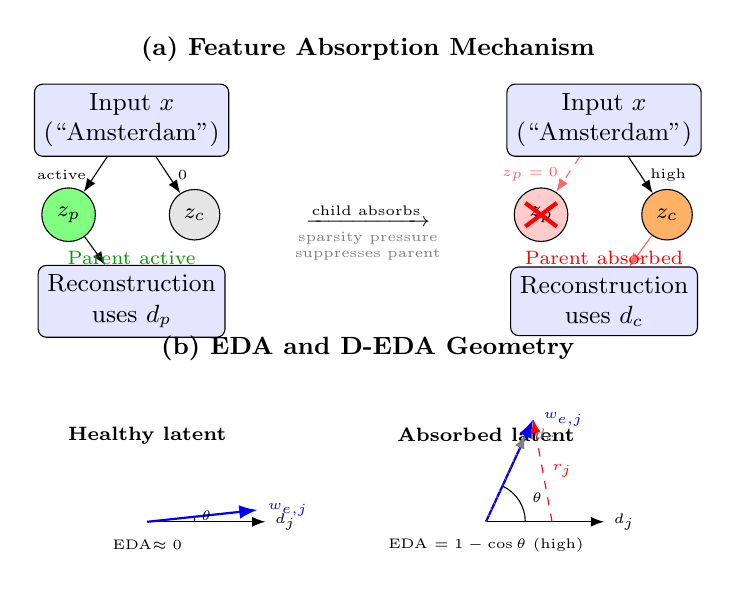
\begin{tikzpicture}[
    node distance=0.6cm and 1.4cm,
    box/.style={draw, rounded corners=3pt, minimum width=1.8cm, minimum height=0.55cm, align=center, font=\small},
    latent/.style={draw, circle, minimum size=0.55cm, font=\footnotesize},
    >=Latex
]

% Panel (a): Feature Absorption Mechanism
\node[font=\small\bfseries] (label_a) at (0, 3.5) {(a) Feature Absorption Mechanism};

% Left: Normal operation
\node[box, fill=blue!10] (x_l) at (-3.0, 2.6) {Input $x$\\(``Amsterdam'')};
\node[latent, fill=green!50] (zp_l) at (-3.8, 1.4) {$z_p$};
\node[latent, fill=gray!20] (zc_l) at (-2.2, 1.4) {$z_c$};
\node[box, fill=blue!10] (recon_l) at (-3.0, 0.3) {Reconstruction\\uses $d_p$};

\draw[->] (x_l) -- (zp_l) node[midway, left, font=\tiny] {active};
\draw[->] (x_l) -- (zc_l) node[midway, right, font=\tiny] {0};
\draw[->] (zp_l) -- (recon_l);
\node[font=\scriptsize, green!60!black, align=center] at (-3.0, 0.85) {Parent active};

% Right: Absorption
\node[box, fill=blue!10] (x_r) at (3.0, 2.6) {Input $x$\\(``Amsterdam'')};
\node[latent, fill=red!20] (zp_r) at (2.2, 1.4) {$z_p$};
\node[latent, fill=orange!60] (zc_r) at (3.8, 1.4) {$z_c$};
\node[box, fill=blue!10] (recon_r) at (3.0, 0.3) {Reconstruction\\uses $d_c$};

\draw[->, dashed, red!60] (x_r) -- (zp_r) node[midway, left, font=\tiny] {$z_p = 0$};
\draw[->] (x_r) -- (zc_r) node[midway, right, font=\tiny] {high};
\draw[->, red!60] (zc_r) -- (recon_r);
\draw[red, line width=1.5pt] (2.0, 1.55) -- (2.4, 1.25);
\draw[red, line width=1.5pt] (2.0, 1.25) -- (2.4, 1.55);
\node[font=\scriptsize, red, align=center] at (3.0, 0.85) {Parent absorbed};

\node[font=\scriptsize, align=center] at (0, 1.4) {$\xrightarrow{\text{child absorbs}}$};
\node[font=\tiny, gray, align=center] at (0, 1.0) {sparsity pressure\\suppresses parent};

% Panel (b): EDA Geometry
\node[font=\small\bfseries] at (0, -0.3) {(b) EDA and D-EDA Geometry};

% Healthy latent
\begin{scope}[shift={(-2.8, -2.5)}]
\node[font=\scriptsize\bfseries] at (0, 1.1) {Healthy latent};
\draw[->] (0,0) -- (1.5, 0) node[right, font=\tiny] {$d_j$};
\draw[->, blue, thick] (0,0) -- (1.4, 0.15) node[right, font=\tiny, blue] {$w_{e,j}$};
\draw (0.6, 0) arc (0:6:0.6);
\node[font=\tiny] at (0.75, 0.08) {$\theta$};
\node[font=\tiny] at (0, -0.3) {EDA$\approx 0$};
\end{scope}

% Absorbed latent
\begin{scope}[shift={(1.5, -2.5)}]
\node[font=\scriptsize\bfseries] at (0, 1.1) {Absorbed latent};
\draw[->] (0,0) -- (1.5, 0) node[right, font=\tiny] {$d_j$};
\draw[->, blue, thick] (0,0) -- (0.6, 1.3) node[right, font=\tiny, blue] {$w_{e,j}$};
\draw[dashed, red, ->] (0.84, 0) -- (0.6, 1.3) node[midway, right, font=\tiny, red] {$r_j$};
\draw[dotted, gray, ->] (0,0) -- (0.5, 1.1) node[right, font=\tiny, gray] {$d_c$};
\draw (0.5, 0) arc (0:65:0.5);
\node[font=\tiny] at (0.65, 0.3) {$\theta$};
\node[font=\tiny] at (0, -0.3) {EDA $= 1-\cos\theta$ (high)};
\end{scope}

\end{tikzpicture}
\caption{(a) Feature absorption: the parent latent $z_p$ (``starts-with-A words'') is suppressed to zero when the child latent $z_c$ (``starts-with-A proper nouns'') is active. The child absorbs the parent's reconstruction contribution. (b) EDA geometry: healthy latents have $w_{e,j}$ aligned with $d_j$ (low EDA); absorbed latents have $w_{e,j}$ rotated toward $d_c$, with residual $r_j$ explained by the absorbing child decoder direction (high EDA).}
\label{fig:mechanism}
\end{figure}

\end{document}
